%! Author = biebl
%! Date = 18.05.2023


\chapter{Anhang}

\section*{Google Trends Weltweiteverteilung von Suchanfragen nach Frameworks}
\begin{figure}[h]
    \centering
    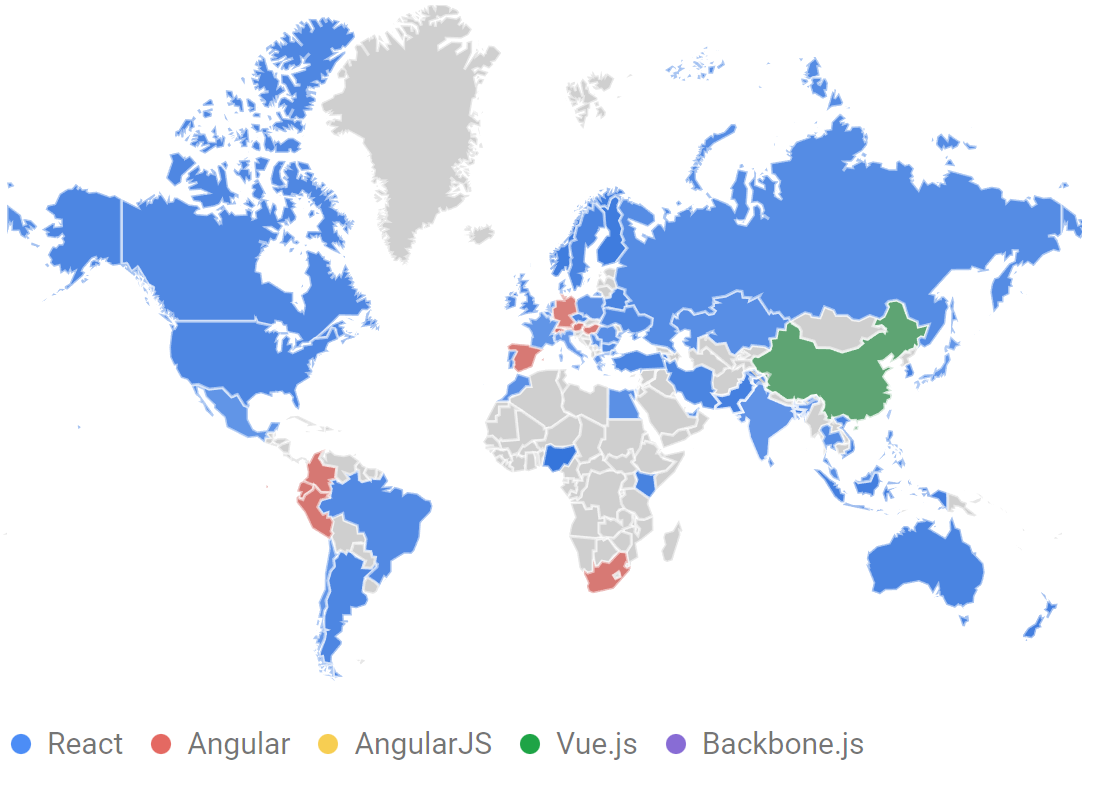
\includegraphics[width=0.8\textwidth]{img/Google Stats/2023-04-26 12_20_26-React, Angular, AngularJS, Vue.js, Backbone.js - Erkunden - Google Trends}
    \caption{Google Trends Weltweiteverteilung von Suchanfragen nach Frameworks der letzten 5 Jahre \cite{googleTrends}}
    \label{fig:google_trends_world}
\end{figure}

\newpage

\section*{Einkaufslistenapp}
\begin{figure}[h]
    \begin{minipage}[H]{.45\textwidth}
        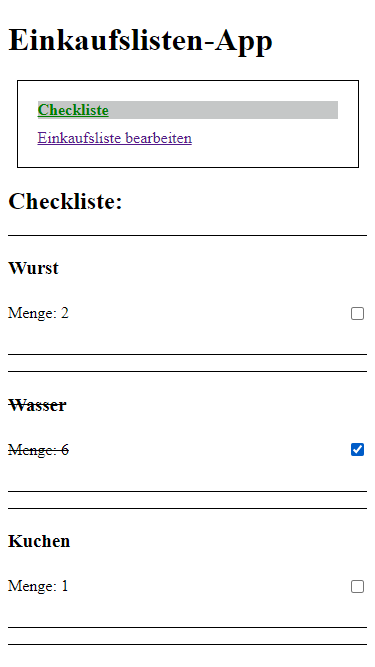
\includegraphics[width=\textwidth]{img/vue-Einkaufsliste-Checkliste}
        \caption{Checklistenseite\\ der Einkaufslistenapp}
        \label{fig:checklistenseite}
    \end{minipage}
    \hspace{.1\linewidth}% Abstand zwischen Bilder
    \begin{minipage}[H]{.45\textwidth}
        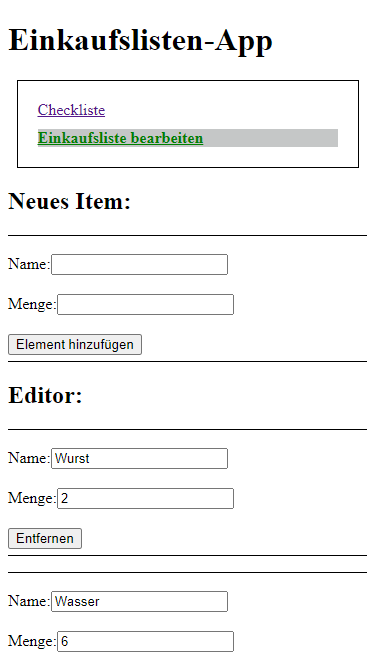
\includegraphics[width=\textwidth]{img/vue-Einkaufsliste-Editor}
        \caption{Bearbeiten- und Erstellenseite der Einkaufslistenapp}
        \label{fig:editlistenseite}
    \end{minipage}
\end{figure}

\textbf{Implementierung mit Angular:} \url{https://github.com/mbbl33/angular-einkaufsliste}
\textbf{Implementierung mit Vue.js:} \url{https://github.com/mbbl33/vue-einkaufsliste}

